\chapter{Plotting with Pyplot}
\label{ch:pyplot}

\section{matplotlib.pyplot}
Matplotlib and its Pyplot environment is a versatile Python plotting
library which produces publication quality figures in a variety of
hard-copy formats such as EPS, PDF, etc.  With PyPlot you can
generate scatter and line plots, histograms, power spectra, bar
charts, error-charts, pie charts, and many more with just a few lines
of code. For the power user, you have full control of line styles,
font properties, and axes properties, etc. For useful examples of 
astronomy plots that can be generated with pyplot, see Leonardo 
Ubeda's astroplotlib library at \href{http://astroplotlib.stsci.edu/}
{http://astroplotlib.stsci.edu/}



\section{Plot with Pyplot}
From Section~\ref{ss:loadtxt} we learned how to read in data from a
file, particularly Gordon2005\_Fig16.txt.  We will reproduce the slope
plot in Figure~16 of the Gordon 2005 paper.

\begin{alltt}
\pytab import numpy as np 
\pytab infile = 'Gordon2005_Fig16.txt' 
\pytab slope, ran_slope_unc, corr_slope_unc, \textbackslash 
\ldots     both_slope_unc, eqn_slope_unc = np.loadtxt(infile, 
\ldots     usecols=(0, 1, 2, 3, 4), unpack=True) 
\end{alltt}

These arrays have nice descriptive names, but to help make the
plotting process clear, we will assign short names.

\begin{alltt}
\pytab xx = slope  
\pytab yy1 = ran_slope_unc  
\pytab yy2 = corr_slope_unc  
\pytab yy3 = both_slope_unc
\pytab yy4 = eqn_slope_unc 
\end{alltt}

Now we will import Pyplot and make our first plot, using a \textit{figure} 
object...

\begin{alltt}
\pytab import matplotlib.pyplot as plt  
\pytab figure, ax = plt.subplots()

Now we can begin to plot 

\pytab plt.plot(xx,yy1)  
\pytab plt.plot(xx,yy1,'b--',xx,yy2,'r:',xx,yy3,'g-', xx,yy4,'m-.')  
\end{alltt}

Notice that `b' is for blue, `r' is for red, `g' is for green, and `m'
is for magenta.  Furthermore, `-' is for a solid line, `--' is for a
dashed line, `:' is for a dotted line, and `-.' is for a dot-dash
line.  Several other options are available as well and can be found on
the PyLab site listed in Chapter~\ref{ch:links}.

The lines are pretty faint, and we also need to add a legend and axis
labels.

\begin{alltt}
\pytab pl.plot(xx,yy1,'b--',xx,yy2,'r:',xx,yy3,'g-',  
\ldots      xx,yy4,'m-.',linewidth=3) 
\pytab pl.legend(('Random Uncertainty',  
\ldots      'Correlated Uncertainty', 'Both','Equation'),'best') 
\pytab pl.ylabel('Slope Unc. [e-/s]')
\pytab pl.xlabel('Slope [e-/s]')
\end{alltt}

We can save this plot.  The figure will save as a PDF, PNG, TIFF, and
others depending on the name given.

\begin{alltt}
\pytab pl.savefig('fig16.pdf')
\pytab pl.clf()
\end{alltt}

Notice that we needed to close the figure.  Open fig16.pdf and take a
look.  It looks pretty good, right?  

\begin{figure}[tbp]
  \centering
    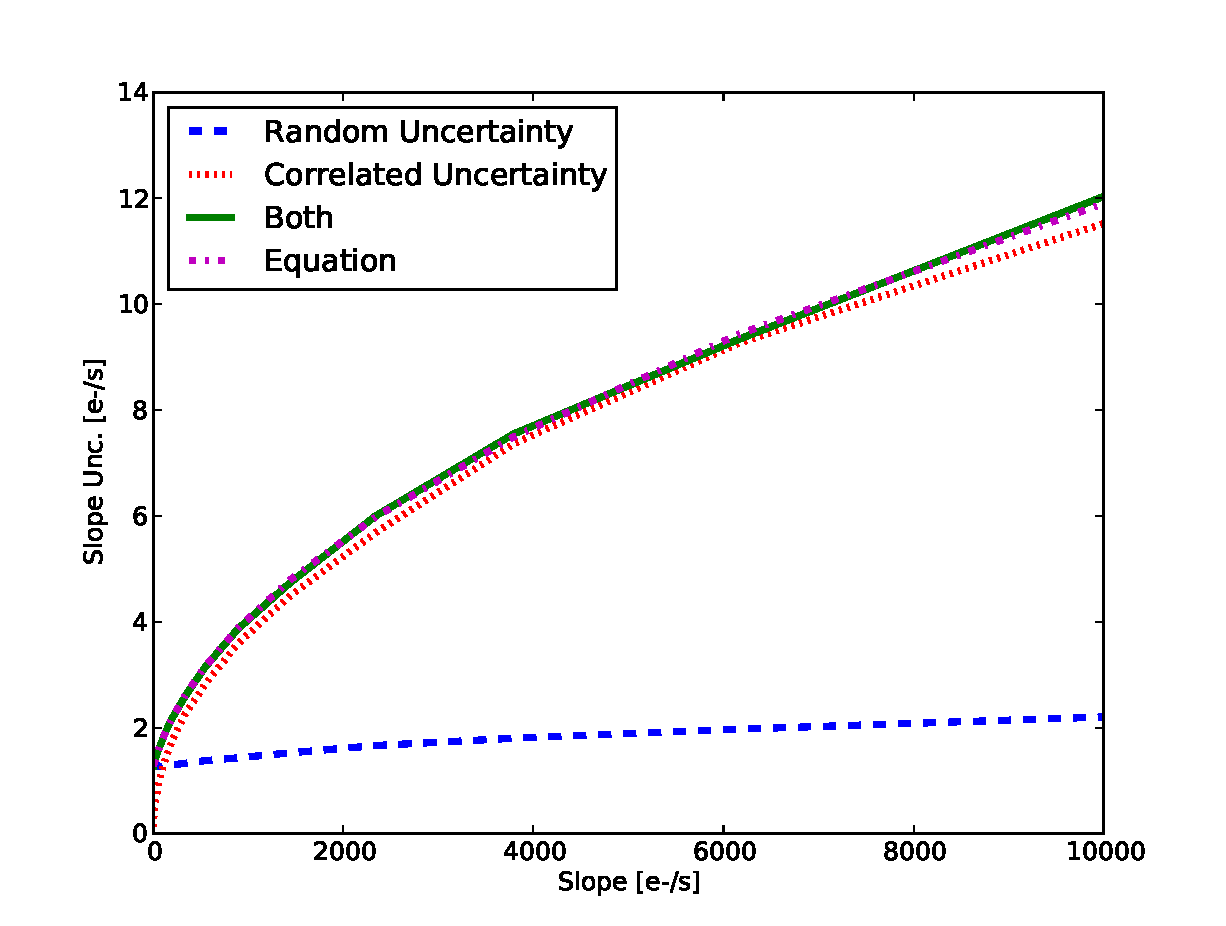
\includegraphics[scale=0.55]{splot.pdf}
    \caption{Our first try at re-creating Figure 16 in Gordon 2005.}
  \label{fig:splot}
\end{figure}

If you look at the paper by
Gordon et al. 2005, you will see that the key thing we are missing is
logarithmic axis.  Instead of {\sf \small pylab.plot} we will use {\sf
\small pylab.loglog}.

\begin{alltt}
\pytab pl.loglog(xx,yy1,'b--',xx,yy2,'r:',xx,yy3,'g-',  
\ldots     xx,yy4,'m-.',linewidth=3) 
\pytab pl.legend(('Random Uncertainty','Correlated Uncertainty',  
\ldots     'Both','Equation'),'best') 
\pytab pl.ylabel('Slope Unc. [e-/s]') 
\pytab pl.xlabel('Slope [e-/s]') 
\pytab pl.savefig('fig16_log.pdf')
\pytab pl.clf()
\end{alltt}

Again, open the figure you just made.  How does that look?  

\begin{figure}[tbp]
  \centering
    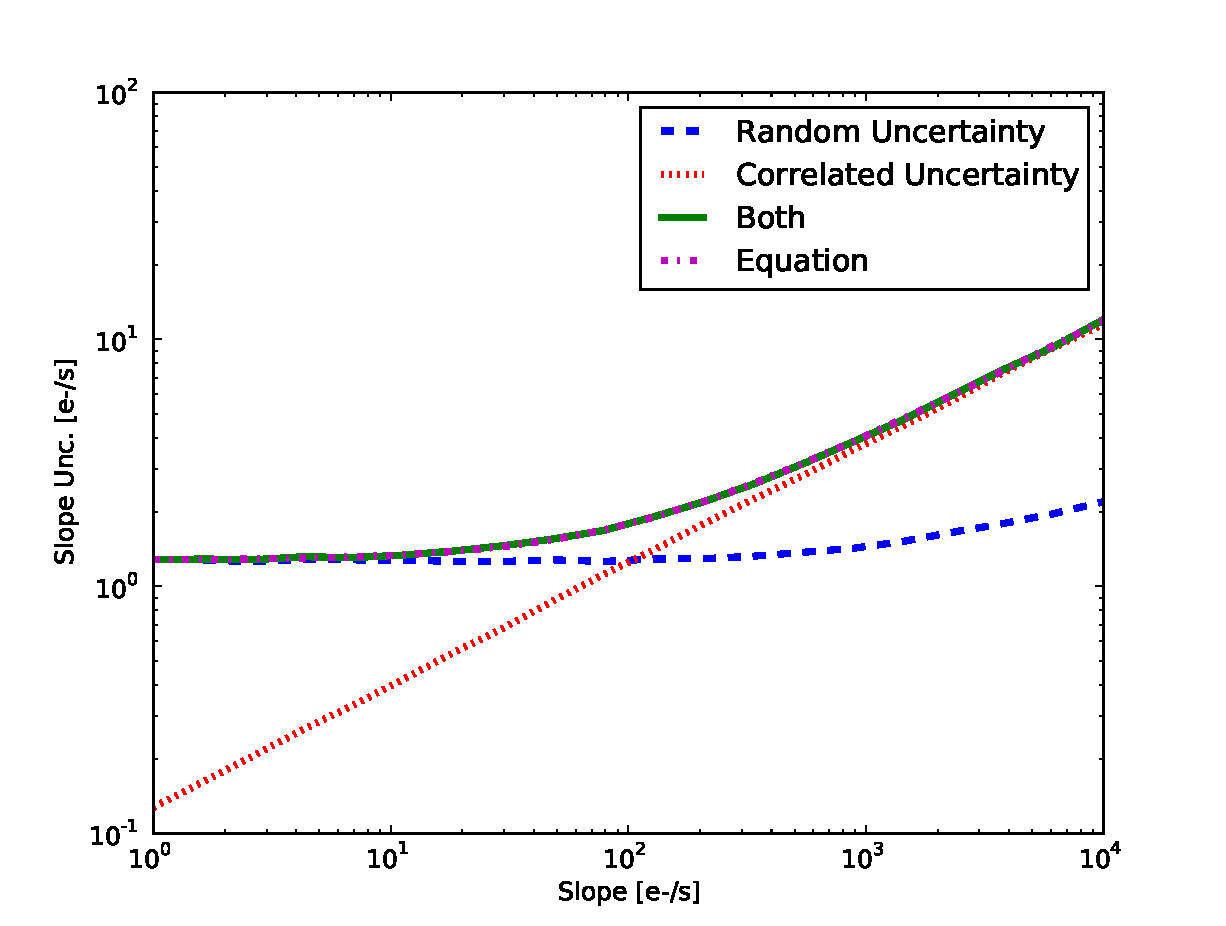
\includegraphics[scale=0.6]{splot_log.pdf}
    \caption{Our version of Figure 16 in Gordon 2005.}
  \label{fig:splot}
\end{figure}

For more
plotting options with Matplotlib and PyLab, check out the link
\url{http://matplotlib.sourceforge.net/} listed in
Chapter~\ref{ch:links}.  Notice that there is a link to NumPy on this
page, as well as links to screen-shots, thumbnails, and examples.

Our plot is looking good, however this is getting way too messy.
Isn't there a way we can keep this all nicely in a file, where we can
type it once correctly and never have to type it again?  Sure there
is!  We need to write a script.
